\documentclass[border=3mm]{standalone}

\usepackage{tikz}
\usetikzlibrary{arrows.meta}

\begin{document}
	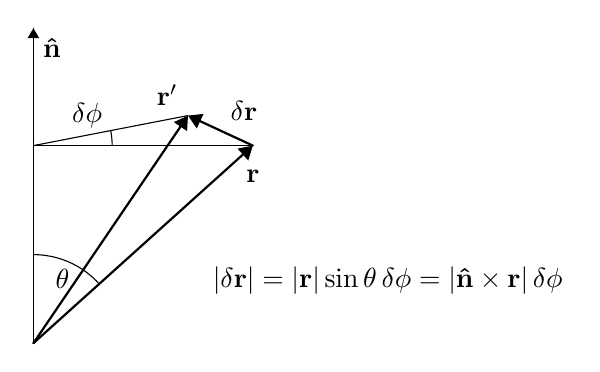
\begin{tikzpicture}[line cap=round]
		\draw[-Triangle] (0,0) -- (0,4) coordinate (a) node[below right] {$\mathbf{\hat{n}}$};
		\draw[thick,-Triangle] (0,0) --++ (42:3.75cm) coordinate (b) coordinate[pos=0.3] (1) node[below,yshift=-5pt] {$\mathbf{r}$};
		\draw (a) -- (a |- b) coordinate (c) -- (b);
		\draw (c) --++ (11:2cm) coordinate (d) coordinate[pos=0.5] (2);
		\draw [thick,-Triangle] (0,0) -- (d) node[above left] {$\mathbf{r'}$};
		\draw[thick,-Triangle] (b) -- (d) node[midway,above right] {$\delta\mathbf{r}$};
		\draw (1) arc (42:90:1.125cm) node[below,pos=0.6]{$\theta$};
		\draw (2) arc (11:0:1cm) node[above left,midway]{$\delta\phi$};
		\node at (4.5,0.8) {$|\delta\mathbf{r}| = |\mathbf{r}|\sin\theta\,\delta\phi = |\mathbf{\hat{n}}\times\mathbf{r}|\,\delta\phi$};
	\end{tikzpicture}
\end{document}